\begin{figure}
\begin{tabular}{cc}
\subfloat[\sffamily{}False negative rate (\%) --- the percentage of \acp{OTU} in the assemblage that were absent from the \softwarename{blast} results following \softwarename{minspec} processing.\label{fig:minspecvalidationfalsenegative}]{
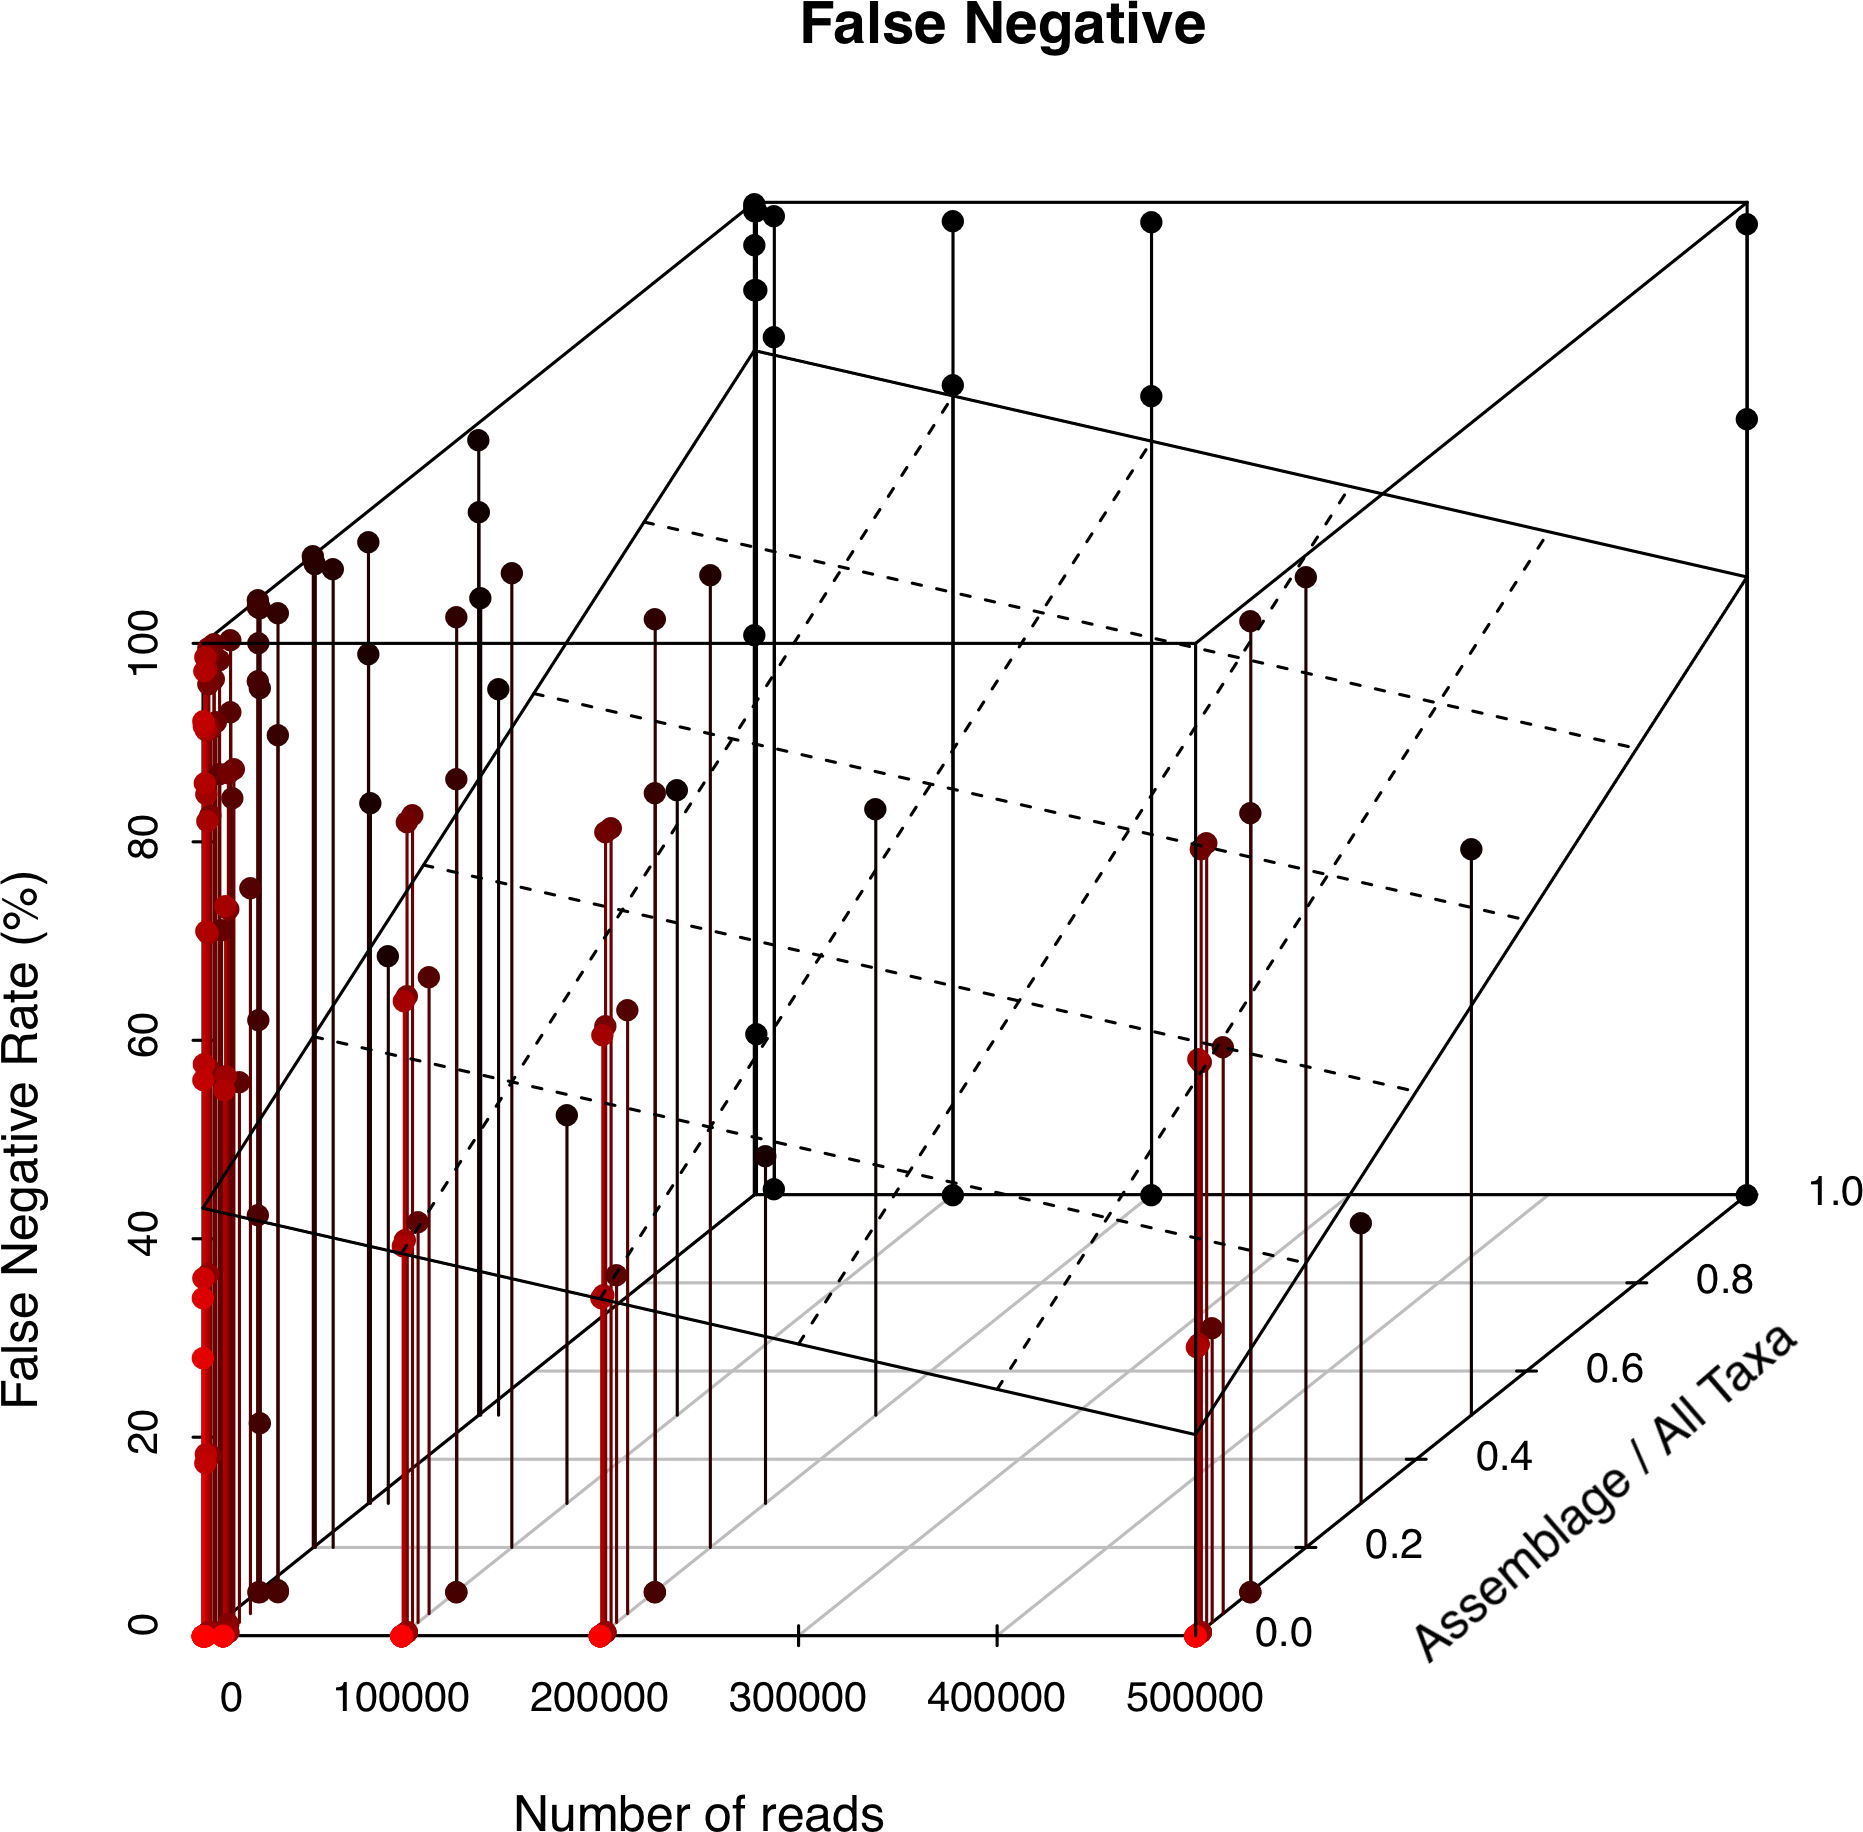
\includegraphics[width=0.45\textwidth]{../minspec/falsenegative.png}
}

&
%\quad %add desired spacing between images, e. g. ~, \quad, \qquad etc. 
%(or a blank line to force the subfigure onto a new line)

\subfloat[\sffamily{}\softwarename{minspec}-attributable false negative rate (\%) --- the percentage of \acp{OTU} not in the assemblage that generated \softwarename{blast} hits but were incorrectly removed by \softwarename{minspec}.\label{fig:minspecvalidationminspecfalsenegative}]{
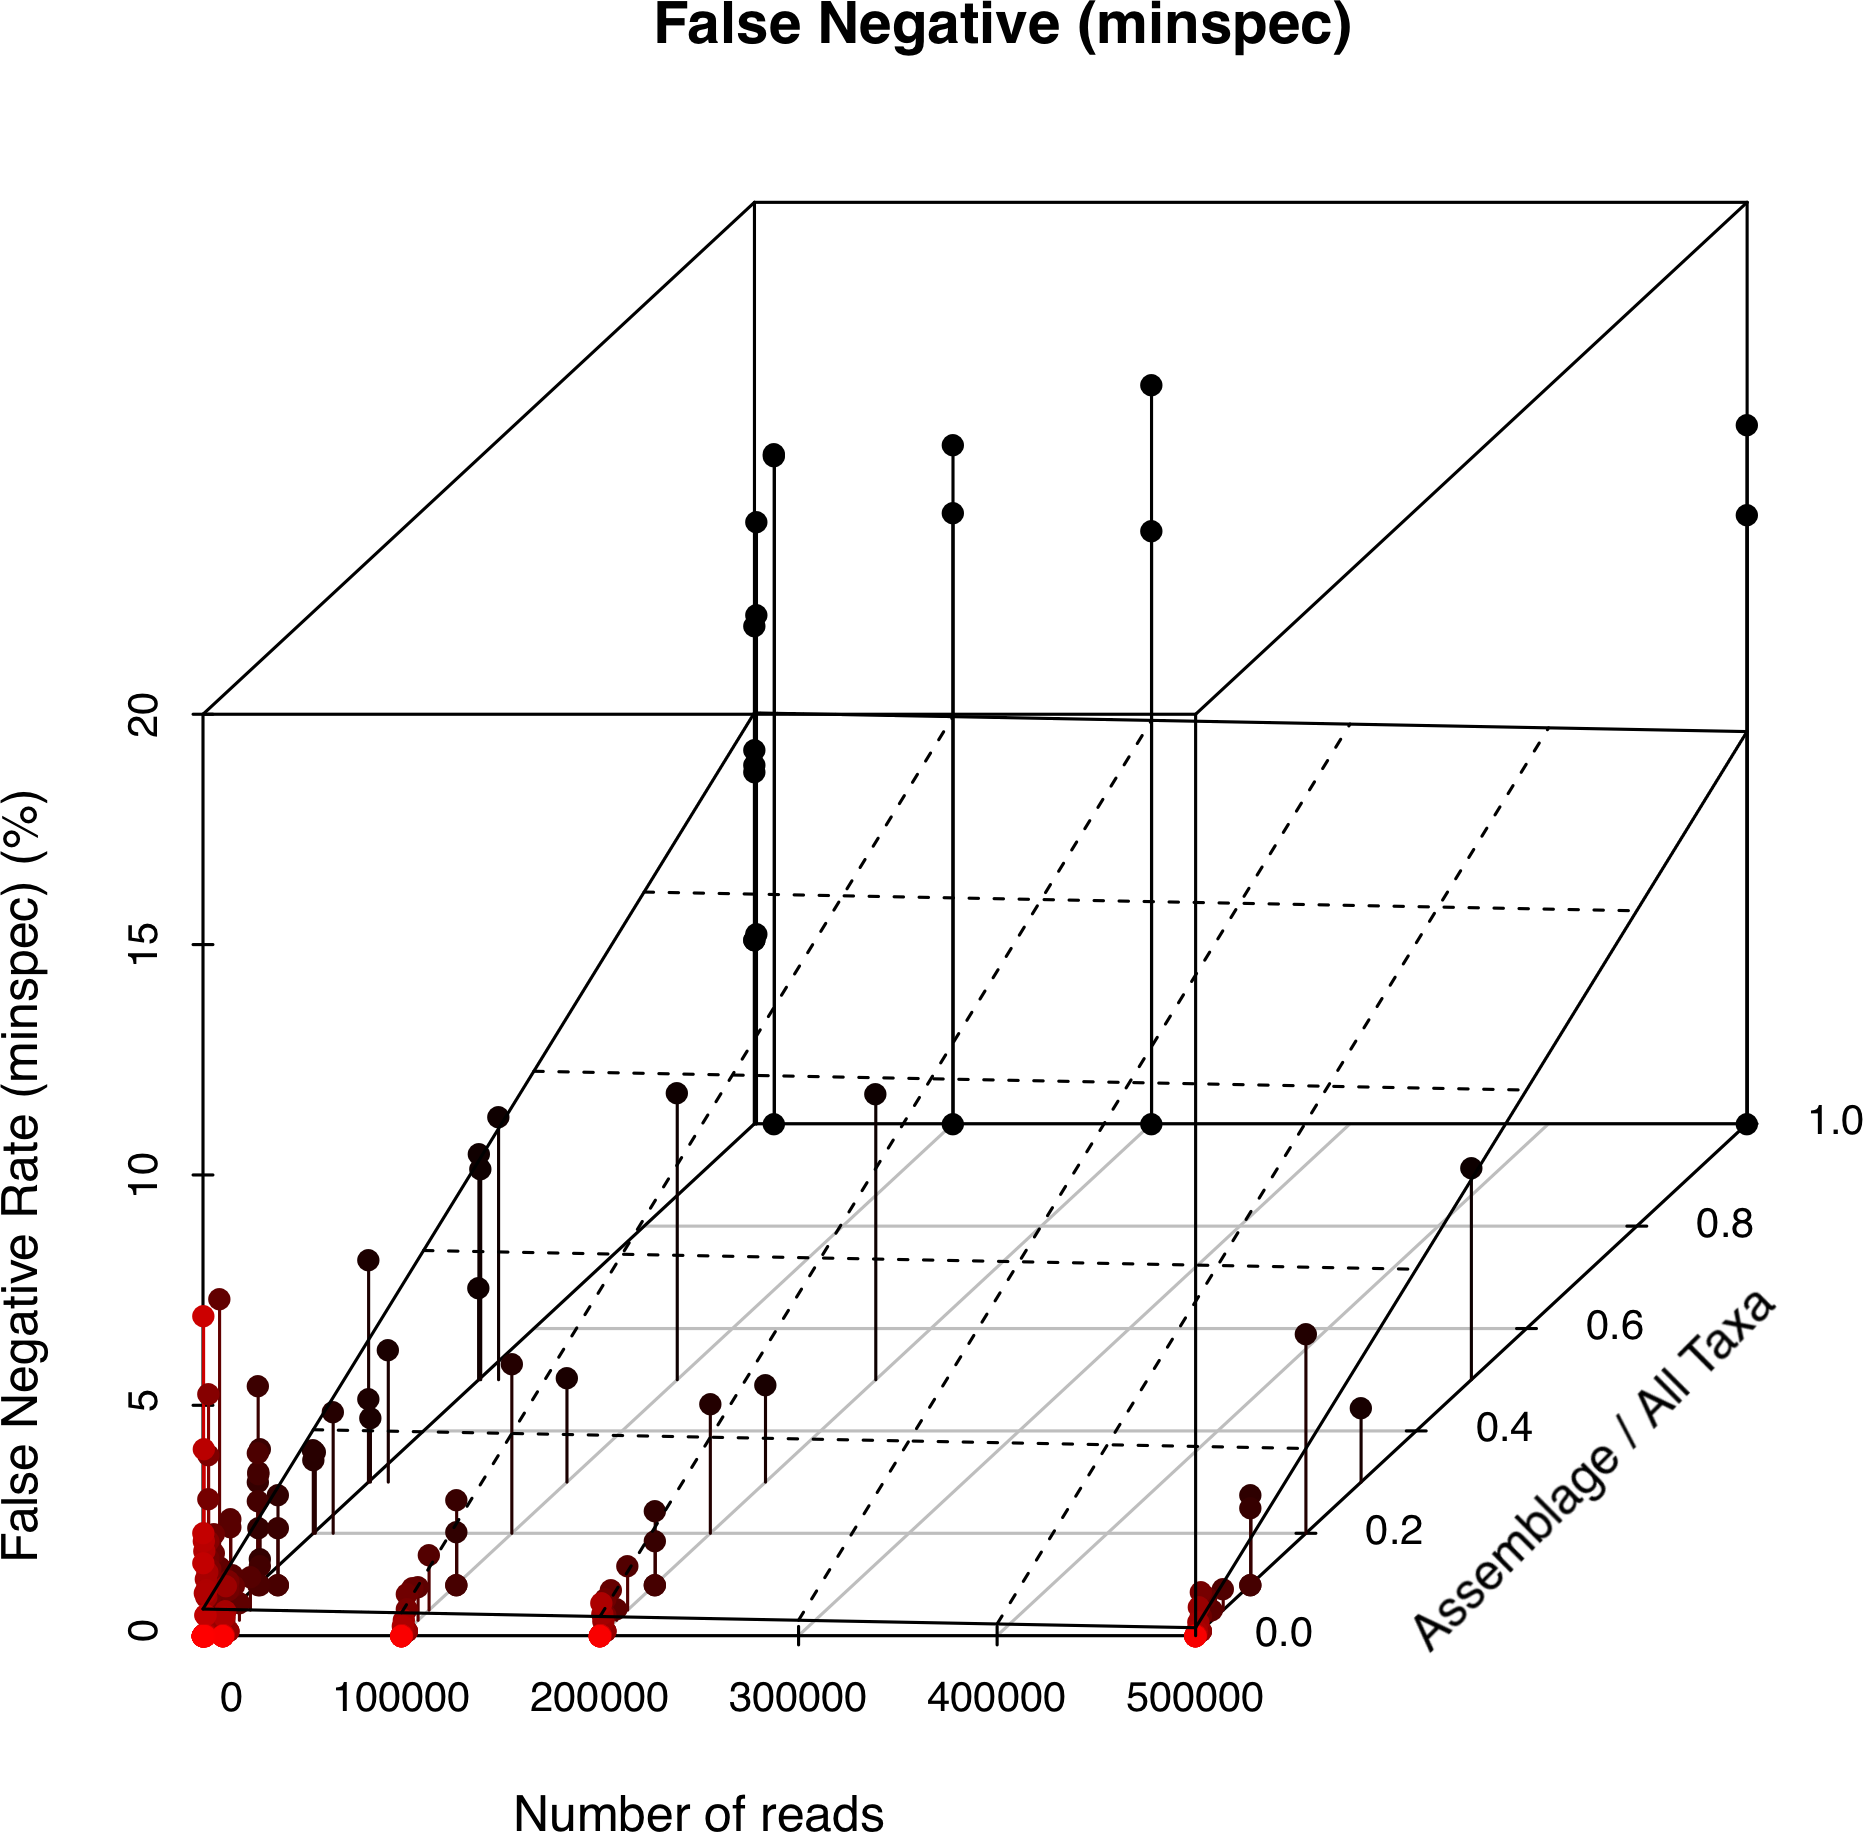
\includegraphics[width=0.45\textwidth]{../minspec/minspecfalsenegative.png}
}
\bigskip
\\
\bigskip
\\
%\quad %add desired spacing between images, e. g. ~, \quad, \qquad etc. 
%(or a blank line to force the subfigure onto a new line)

\subfloat[\sffamily{}False positive rate (\%) --- the percentage of \acp{OTU} not in the assemblage that were present in the \softwarename{blast} results following \softwarename{minspec} processing. \label{fig:minspecvalidationfalsepositive}]{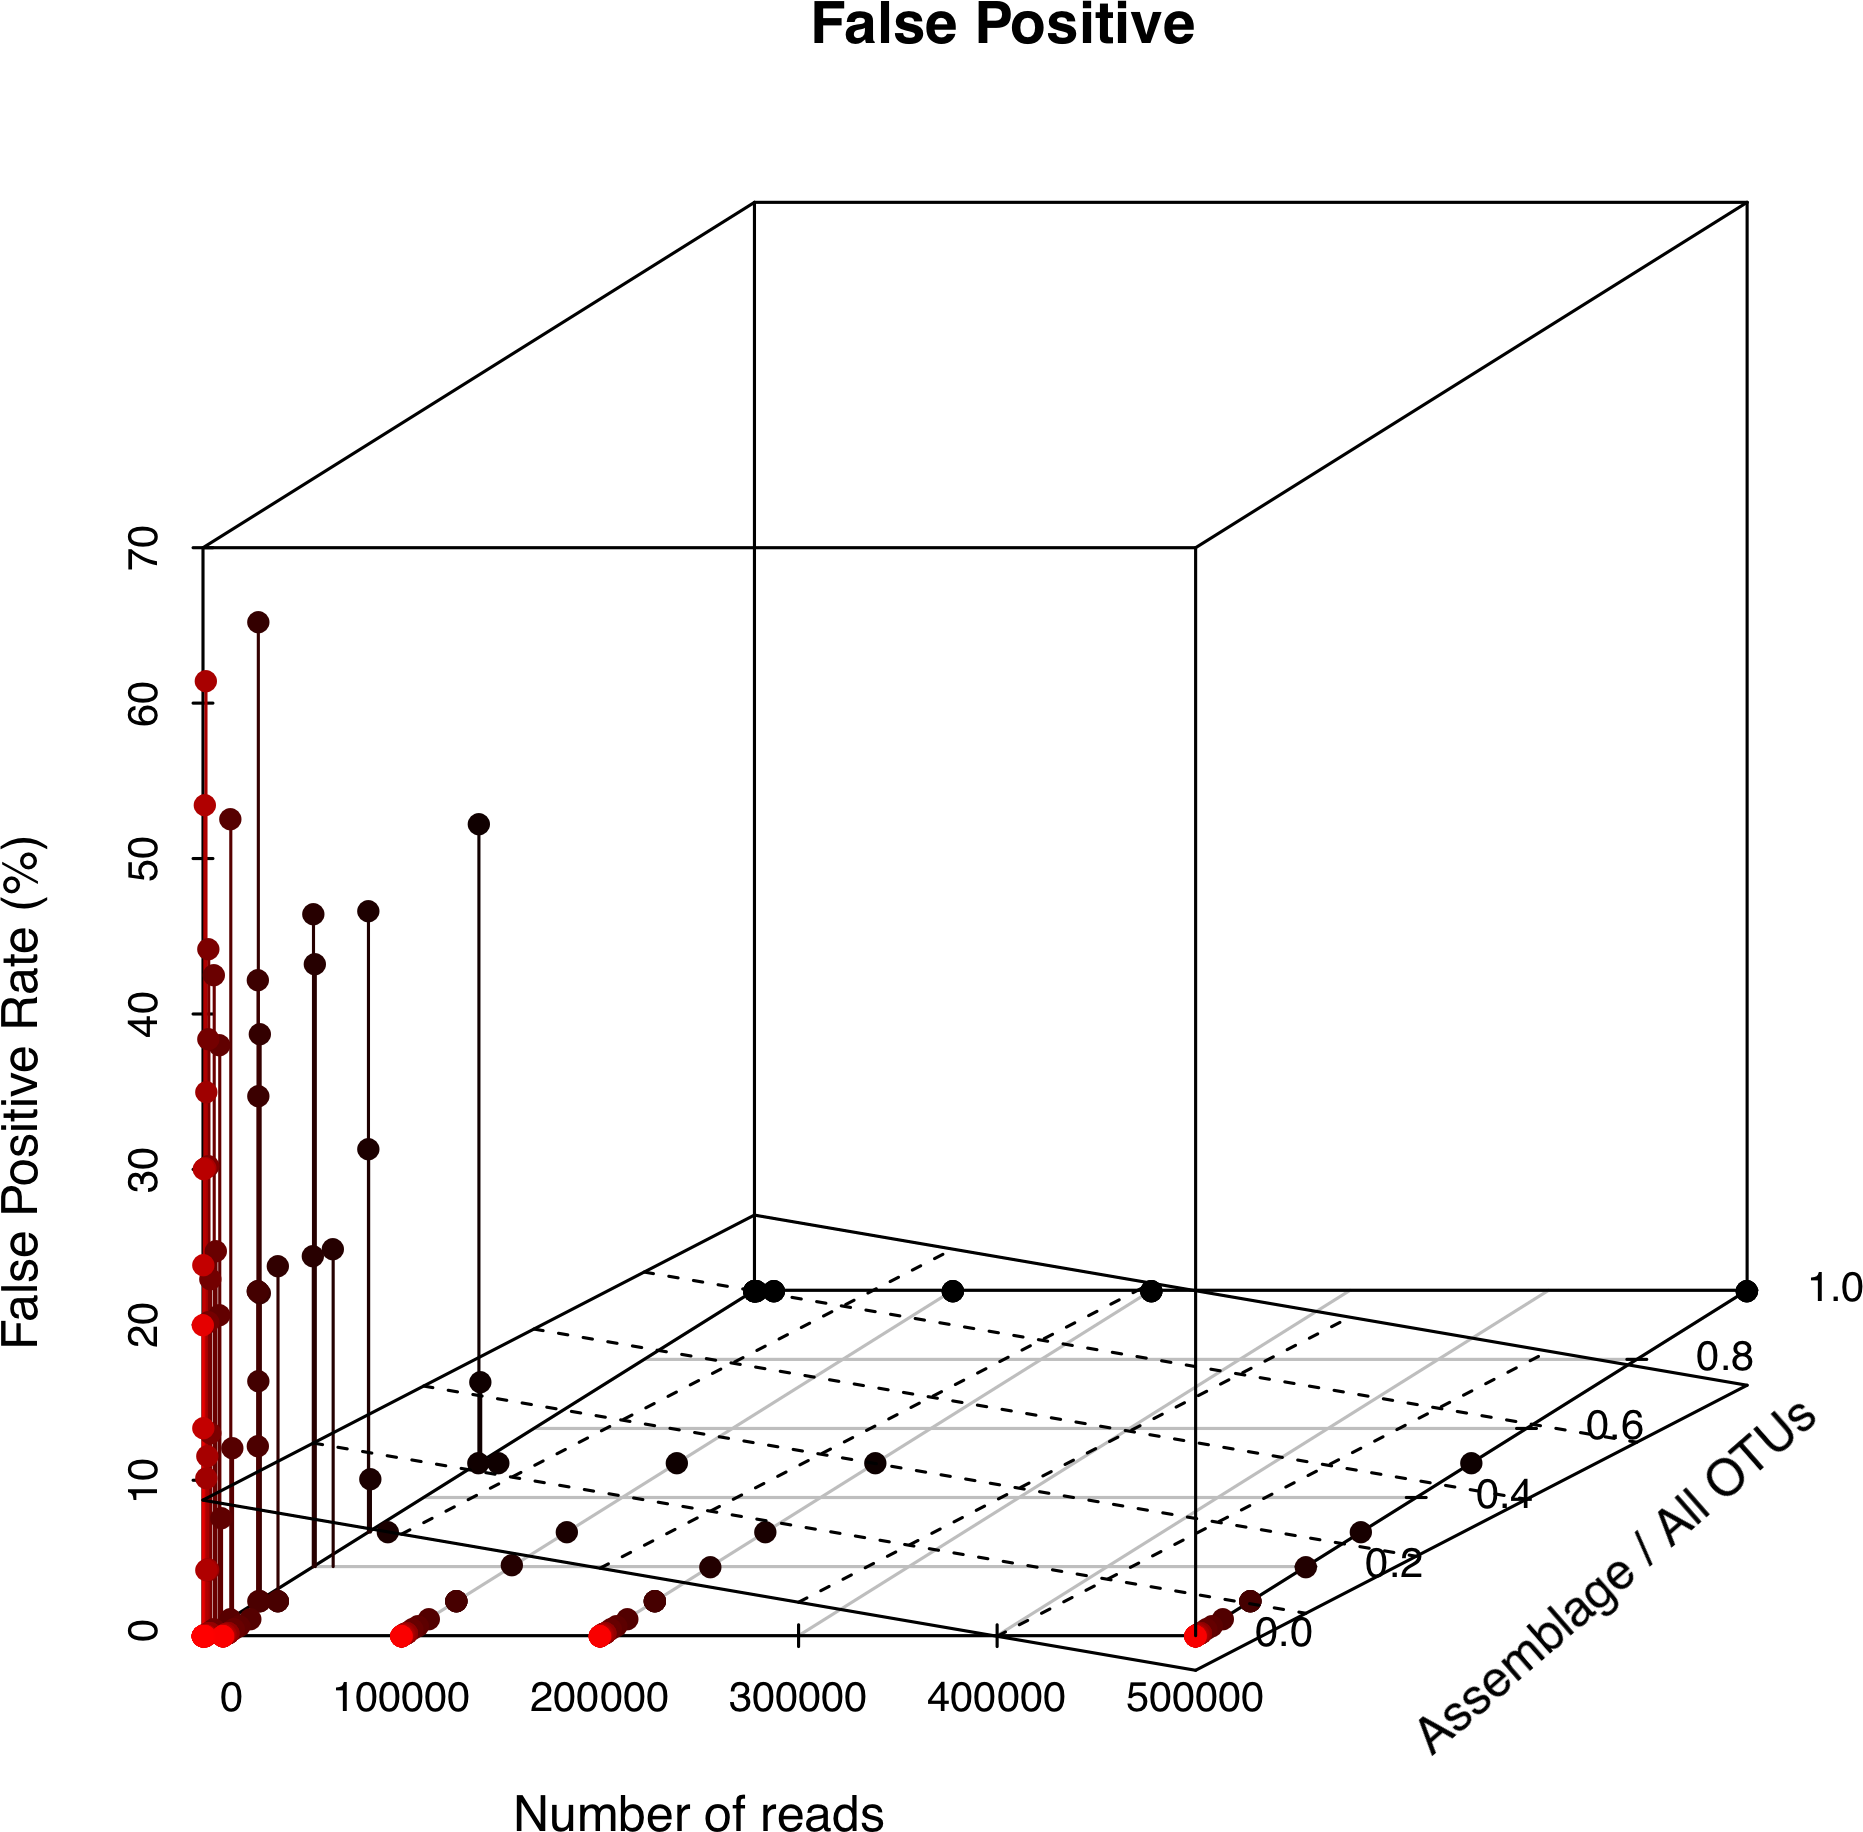
\includegraphics[width=0.45\textwidth]{../minspec/falsepositive.png}}

&
%\quad %add desired spacing between images, e. g. ~, \quad, \qquad etc. 
%(or a blank line to force the subfigure onto a new line)

\subfloat[\sffamily{}Proportion of false \acp{OTU} --- \acp{OTU} that were not part of the simulated assemblage but which generated hits due to simulated sequence identity --- that were correctly identified and removed by \softwarename{minspec}.\label{fig:minspecvalidationfalseotusremoved}]{
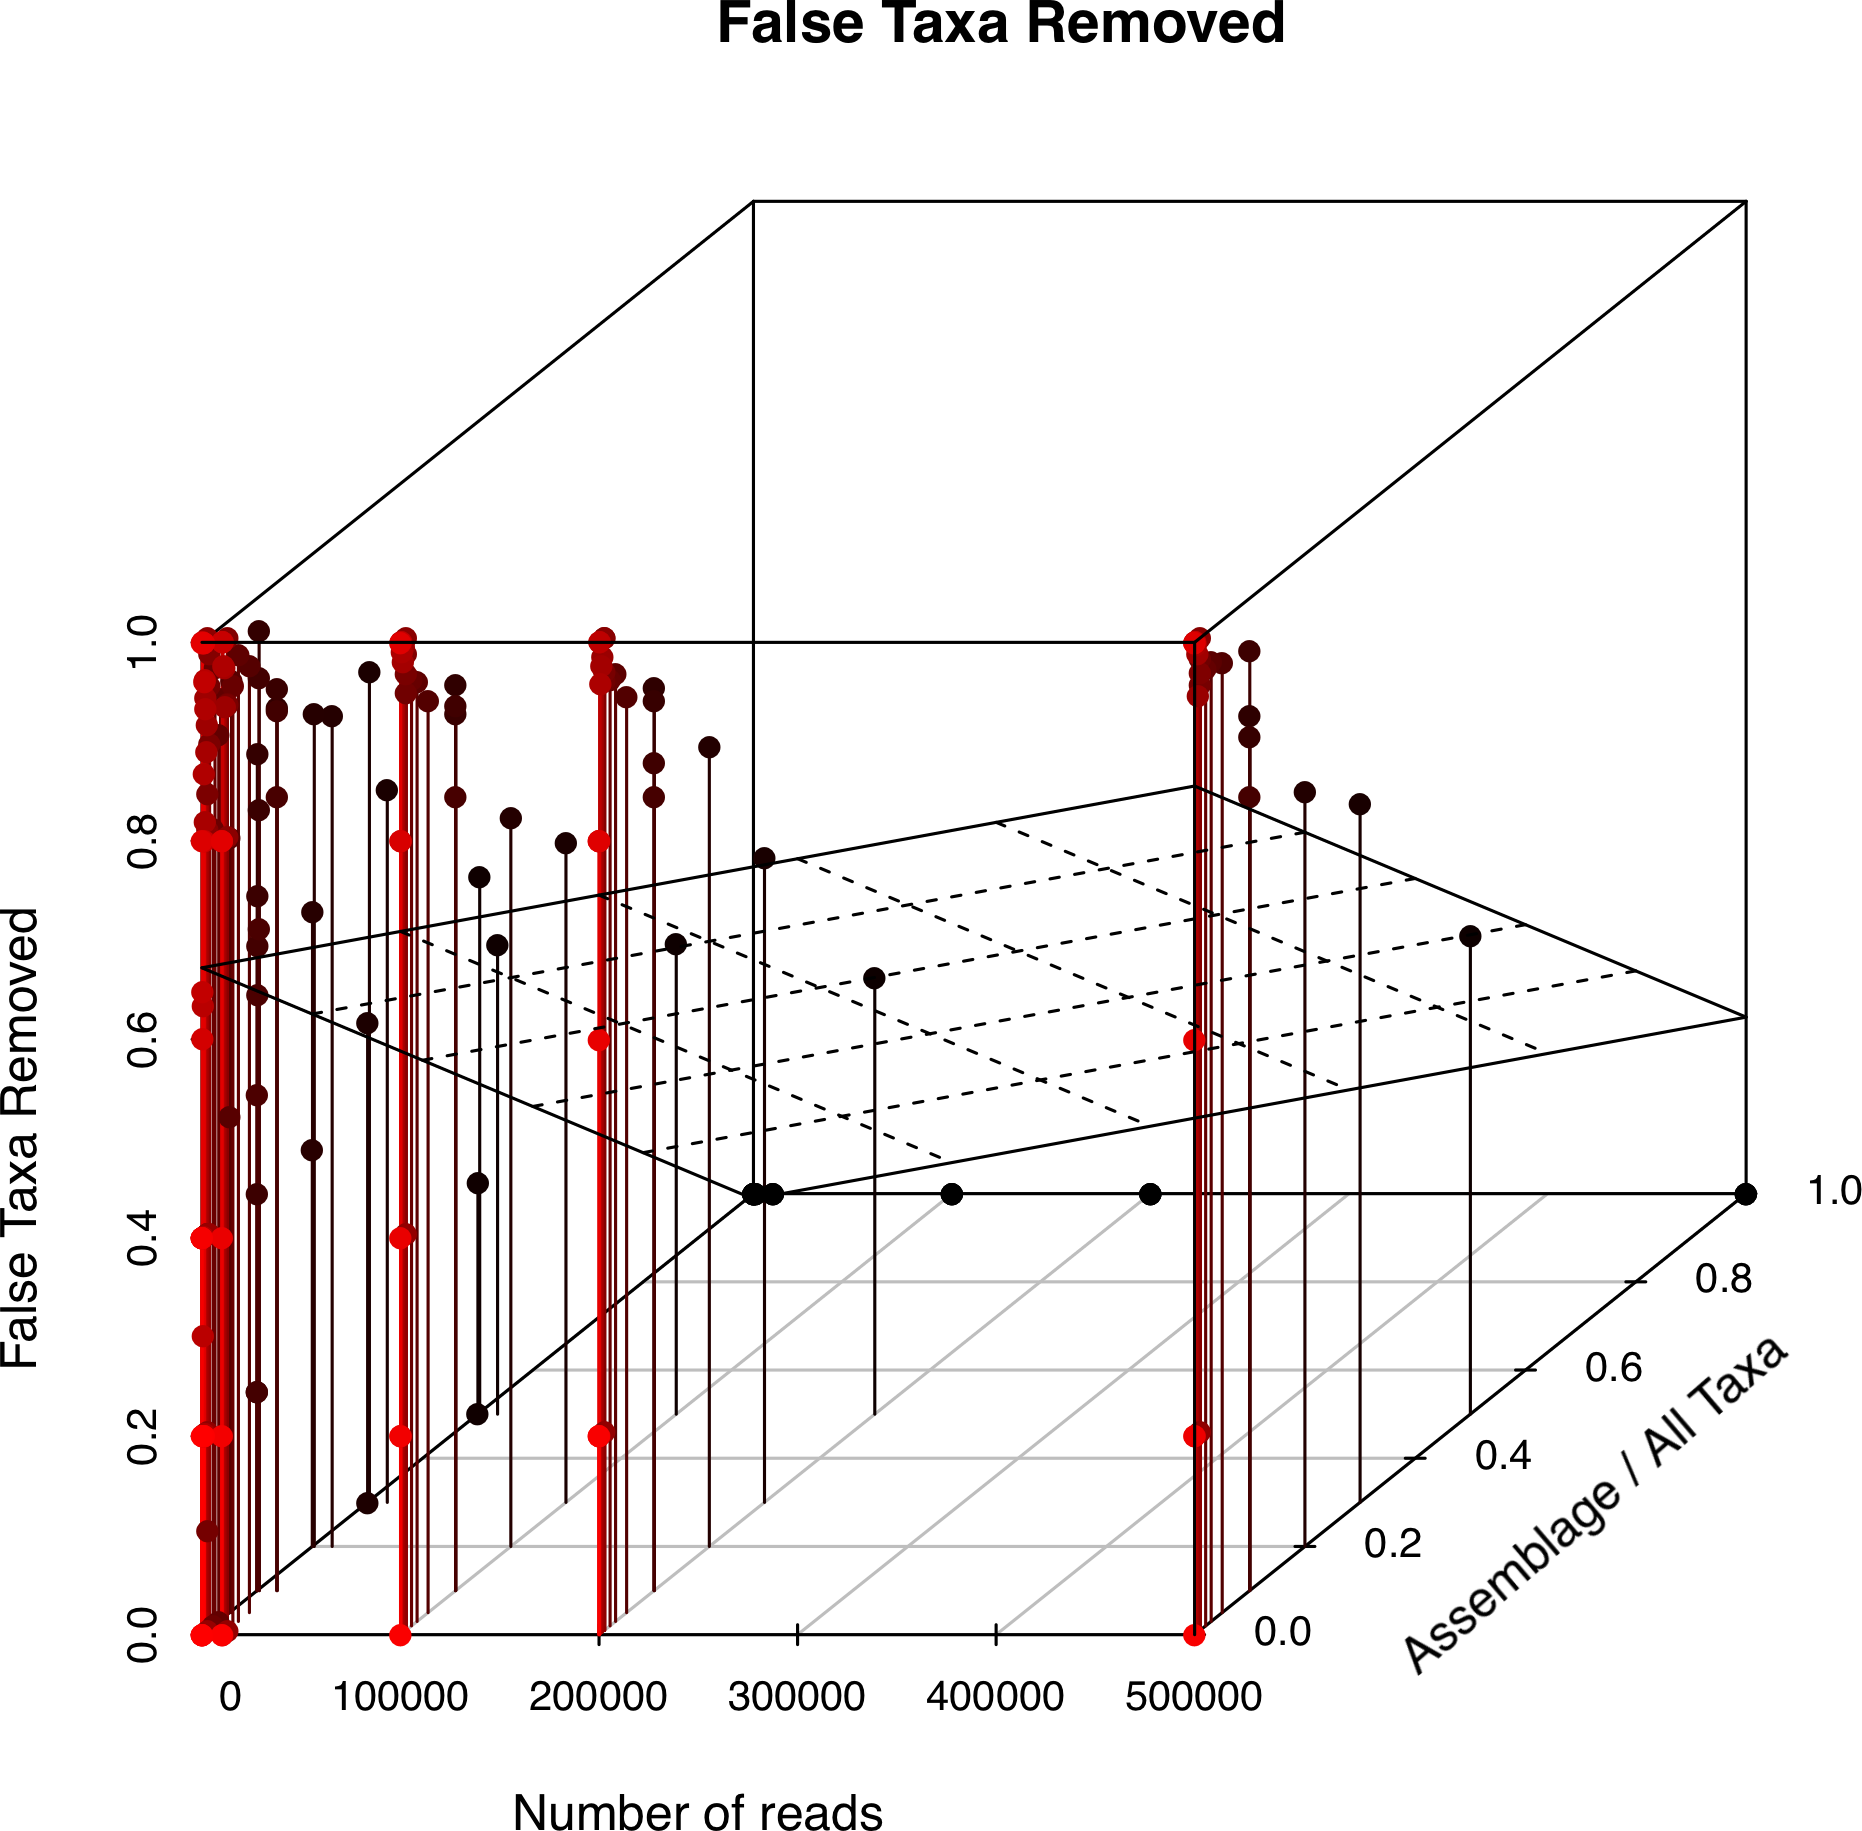
\includegraphics[width=0.45\textwidth]{../minspec/falseotusremoved.png}
}
\\

\end{tabular}

\caption[Results of \softwarename{minspec} validation]{Results of repeated trials of \softwarename{minspec} on simulated metagenomic studies with multiple permutations of parameters (number of reads, number of simulated \acp{OTU}, size of simulated assemblage).
The number of simulated \acp{OTU} and size of simulated assemblage are represented as a ratio on the z-axis (``assemblage / all \acp{OTU}'').
Each permutation was repeated five times.
A plane representing a linear regression has been overlaid on each plot to indicate the trend.
Points have been tinted to aid the perception of depth; colour is not otherwise meaningful.
}\label{fig:minspecvalidation}
\end{figure}
